%--------------------------------------------------------------------------------
%\documentclass{article}

\documentclass[a4paper, 12pt]{article}
\usepackage[T1]{fontenc} 
\usepackage[bf]{caption}
\usepackage{hyperref}
\usepackage[all]{hypcap}
\usepackage[utf8]{inputenc}
\usepackage{graphicx}
\usepackage[czech, english]{babel}
\selectlanguage{czech}
\usepackage{subfig}                % \subfloat
\usepackage{color}
\usepackage{url}
\usepackage{float}
\inputencoding{utf8}
%\usepackage[bf]{caption2}
\usepackage{hyperref}
\usepackage[all]{hypcap}
\hypersetup{colorlinks=false, linkbordercolor=1 1 1, citebordercolor=1 1 1}
\usepackage[right]{lineno}
\renewcommand\linenumberfont{\normalfont\tiny\color{blue}}


\title{Dokumentace projektu PGP}
\author{
	Vít Hodes\\
	\texttt{xhodes00@stud.fit.vutbr.cz}
	\and
	Zdeněk Biberle\\
	\texttt{xbiber00@stud.fit.vutbr.cz}
}
\date{\today}


%--------------------------------------------------------------------------------


\begin{document}
\selectlanguage{czech}
\maketitle

\section{Úvod}


Tato práce se zabývá implementací algoritmu Real Time Shadow of Transparent Casters Using Shadow
Volume popsaný v \cite{Byungmoon2007}. Tento algoritmus, jak již jeho název naznačuje, popisuje způsob řešení stínů pomocí objemových těles, aplikovatelný i
na neuzavřené modely a tedy i obecné trojuhelníky - tzv. triangle soup. Dále algoritmus popisuje
postup tvorby stínů průhledných casterů a jejich nedokonalosti a možná řešení.

%%%%%%%%%%%%%%%%%%%%%%%%%%%%%%%%%%%%%%%%%%%%%%%%%%%%%%%%%%%%%%%%%%%%%%%%%%%%%%%%%%%%%%%%

\section{Teorie}

Klíčovou částí algoritmu popsaného v \cite{Byungmoon2007} je zjištění intenzity světla po průchodu stínícím tělesem. Naivní způsob, kterým lze toto provést, je vytvoření stínového tělesa pro každý trojúhelník stínícího tělesa a následná aplikace typického shadow-volume algoritmu z-pass či z-fail.

\begin{figure}[H]
	\centering
	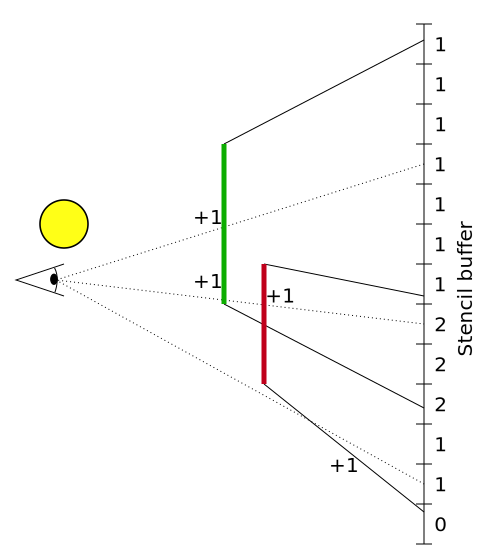
\includegraphics[width=10cm,keepaspectratio]{basic-shadow-volumes}
	\caption{Základní myšlenka více stínových těles}
	\label{fig:basic-shadow-volumes}
\end{figure}

Po této operaci získáme stencil buffer, jehož hodnoty pro každý pixel framebufferu určují počet ploch, skrz které prošel světelný paprsek.

Pokud předpokládáme, že každá z těchto ploch propouští stejné množství světla, tak můžeme intenzitu světla dopadajícího na objekty následujícím způsobem:

\begin{equation}
	I_{out} = f^s * I_{in}
\end{equation} 

kde $I_{out}$ je celková intenzita světla, $I_{in}$ je intenzita zdroje světla, $f$ je faktor propustnosti stínícího objektu a $s$ je hodnota stencil bufferu na patřičné pozici. Tento postup lze jednoduše rozšířit na všechny barevné kanály.

Nevýhodou tohoto naivního přístupu je značné množství vykreslovaných stínových těles a mnoho operací se stencil bufferem. Omezení počtu stínových těles je možné provést na základě myšlenky je demonstrováno na obrázku \ref{fig:joining-shadow-volumes}. Obecně lze říci, že z hrany je nutné protáhnout stěnu stínového tělesa pouze v případě, že na obou stranách protažené hrany je stejný počet trojúhelníků, které tuto hranu sdílí. Pokud je tento počit odlišný, tak hranu protáhneme a přiřadíme jí tzv. multiplicitu, tedy rozdíl počtu trojúhelníků na obou stranách.

\begin{figure}[H]
	\centering
	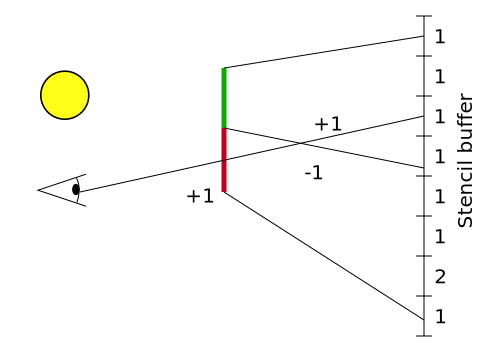
\includegraphics[width=10cm,keepaspectratio]{joining-shadow-volumes}
	\caption{Ukázka nadbytečných stěn stínových těles}
	\label{fig:joining-shadow-volumes}
\end{figure}


%%%%%%%%%%%%%%%%%%%%%%%%%%%%%%%%%%%%%%%%%%%%%%%%%%%%%%%%%%%%%%%%%%%%%%%%%%%%%%%%%%%%%%%%

\section{Popis řešení}


Bylo implementováno referenční CPU řešení, které bylo převáděno do compute a geometry shaderů.
Řešení se skládá prakticky ze dvou částí - spočítání objemových těles zvolenou metodou a poté
samotný proces vygenerování stínů a vykreslení.

Na začátku se předzpracují modely tak, že se odstraní duplikované vrcholy a vygenerují se nové
vertex a element vektory. Pak se vygeneruje tzv. edgeLookup vektor, ve kterém se z trojuhelníků 
vytvoří seřazená množina hran s třetím nehranovým vrcholem a id trojuhelníku. Hrany jsou seřazeny
 podle vrcholu 1, pak vrcholu 2 a nakonec podle id trojuhelníku. Takto seřazený vektor umožňuje vyhledání všech trojúhelníků náležících k dané hraně v logaritmickém čase.

Implementace algoritmu se v jednotlivých implementacích příliš neliší. Ve všech případech jsou na
vstupu vrcholy modelu, element vektor definující jednotlivé trojühelníky, edgeLookup, pozice světla a 
požadovaná délka extrudovaného stínu. V compute a geometry shaderech jsou tyto data v SSBO bufferech
(kromě pozice světla a délky stínu - ty jsou obyčejné uniformy).
 
Pro každý trojúhelník, pokud je přivrácený ke světlu, se vygeneruje nový extrudovaný o příslušnou vzdálenost
od světla. Pro každou jeho hranu se naleznou všechny trojühelníky, které tuto hranu sdílí, a podle jejich orientace se nastaví multiplicita hrany (tj. zda stín generuje či nikoliv).
Pokud je výsledná multiplicita nenulová, vytvoří se z příslušné hrany stěna objemového tělesa.



Postup kreslení začíná vykreslením stíněných povrchů do hloubkového bufferu, který je použitý při 
z-fail generování ``stencil'' textury stínů. Při z-fail algoritmu je zápis do hloubkového bufferu vypnutý
a pro každý fragment, který má hloubku větší než je aktuální v hloubkovém bufferu, atomicky zapíše negativní
hodnotu své multiplicity (pro fragmenty orientované od kamery je tato hodnota ve výsledku kladná a pro
fragmenty orientované ke kameře záporná) do celočíselné ``stencil'' textury. Je také zapnutý early fragment test,
jinak by atomické operace proběhly i pro fragmenty, které se budou zahazovat.

Se získanou texturou se stínem už stačí vykreslit znovu stíněné předměty a poté stínící předměty bez ní.

\subsection{Zajímavé řešené problémy}
Pro atomické load/store operace jsou podporovány pouze celočíselné formáty textur r32i a r32ui.
AMD má opravdu problém s přímým využitím hodnot ze SSBO pole, ale zkopírování do pomocné proměnné tento problém obejde.
Padding vstupních dat je opravdu potřeba. Dlouho nás ani nenapadlo tam hledat chybu a vůbec se tím zabývat. 

%%%%%%%%%%%%%%%%%%%%%%%%%%%%%%%%%%%%%%%%%%%%%%%%%%%%%%%%%%%%%%%%%%%%%%%%%%%%%%%%%%%%%%%%

\section{Ovládání}

\begin{itemize}
	\item T - zapne vykreslování objemových těles
	\item C - přepíná mezi metodami generování objemových těles
	\item I - zapne zobrazení statistik běhu programu
	\item R - zastaví rotaci scény
	\item B - přepnutí stínícího modelu
	\item Myš - rotace okolo počátku scény
	\item Kolečko - přiblížení/oddálení pohledu ve scén?
	\item Esc - ukončí běh openGL programu, Enter potom celé aplikace
\end{itemize}

%%%%%%%%%%%%%%%%%%%%%%%%%%%%%%%%%%%%%%%%%%%%%%%%%%%%%%%%%%%%%%%%%%%%%%%%%%%%%%%%%%%%%%%%

\section{Vyhodnocení}

I přes problémy s AMD hardwarem se nakonec podařilo implementaci v compute i geometry shaderech zprovoznit.
Problémy byly v paddingu vstupních struktur i samotné implementaci algoritmu, kde se počítaly
některé trojuhelníky navíc. 

\begin{figure}[H]
	\centering
	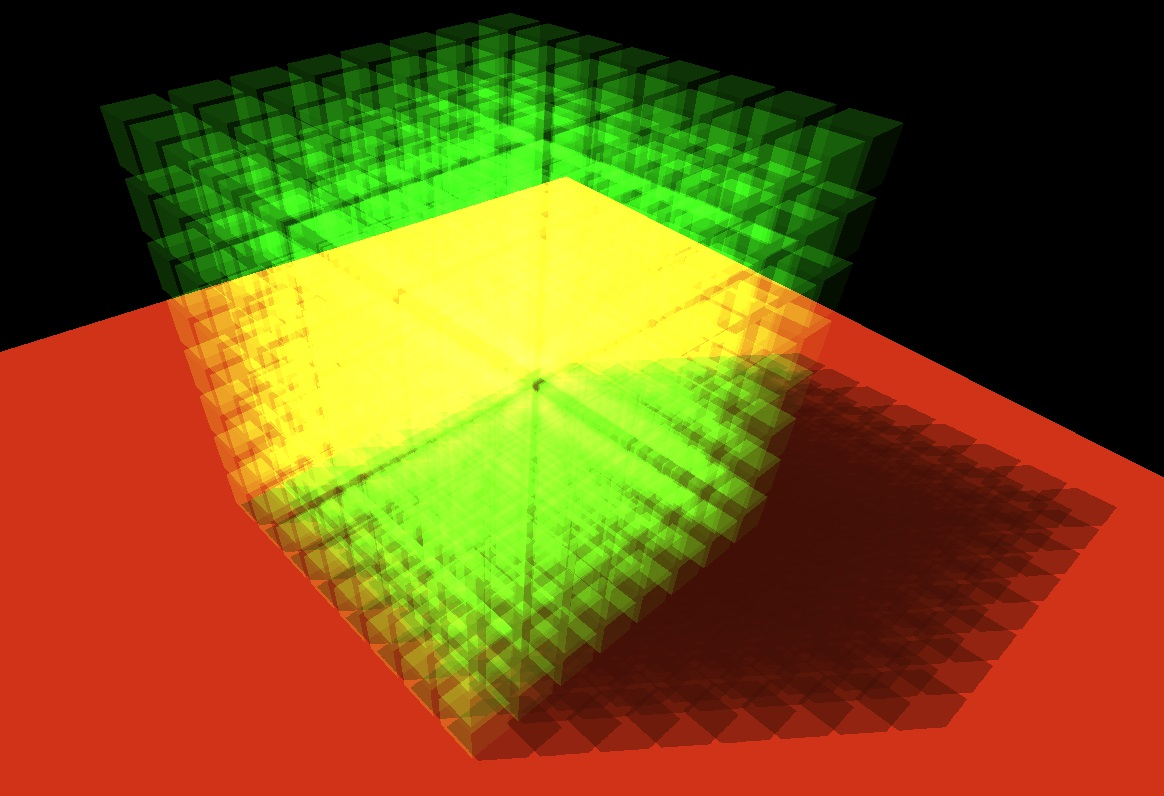
\includegraphics[width=12cm,keepaspectratio]{screenshot}
	\caption{Screenshot aplikace}
	\label{fig:screenshot}
\end{figure}

Měření výkonu bylo prováděno na počítači s procesorem Intel i5 4670K a grafickou kartou AMD Radeon 280X. Měření byla provedena se všemi metodami ve dvou různých rozlišeních s následujícími modely:

\begin{itemize}
	\item plane - Jednoduchá rovina tvořená ze dvou trojúhelníků.
	\item bunny - Běžný Stanford Bunny, 4968 trojúhelníků.
	\item cubes - 512 krychlí, 6144 trojúhelníků.
\end{itemize}

Výsledky měření jsou v grafech \ref{fig:mereni-1024} a \ref{fig:mereni-1920}.

\begin{figure}[H]
	\centering
	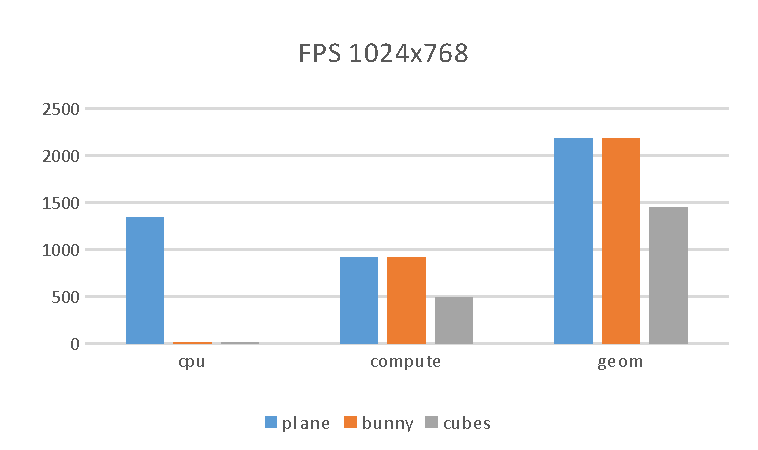
\includegraphics[width=12cm,keepaspectratio]{mereni-1024}
	\caption{Výsledky měření při rozlišení $1024\times768$}
	\label{fig:mereni-1024}
\end{figure}

\begin{figure}[H]
	\centering
	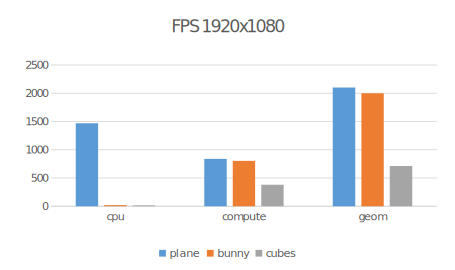
\includegraphics[width=12cm,keepaspectratio]{mereni-1920}
	\caption{Výsledky měření při rozlišení $1920\times1080$}
	\label{fig:mereni-1920}
\end{figure}

%%%%%%%%%%%%%%%%%%%%%%%%%%%%%%%%%%%%%%%%%%%%%%%%%%%%%%%%%%%%%%%%%%%%%%%%%%%%%%%%%%%%%%%%

\section{Závěr}

Výsledky jsou v mnoha případech dle očekávání -- korektně funguje stínování závislé na počtu stěn, kterými světlo prochází. Algoritmus z-fail taktéž funguje.

Zajímavý je ovšem podstatně nižší výkon compute shaderů oproti geometry shaderům.

\bibliographystyle{czechiso}
\begin{flushleft}
  \bibliography{project}
\end{flushleft}

%\appendix
%\newpage
%\section{}

\end{document}
